\documentclass[border=0pt]{standalone}
\usepackage{pgfplots}
\pgfplotsset{width=\linewidth,compat=1.8}
\usepackage{pgfplotstable}
\usepgfplotslibrary{fillbetween}
\usepackage{amsmath}
\begin{document}

\pgfplotsset{every tick label/.append style={font=\boldmath}}

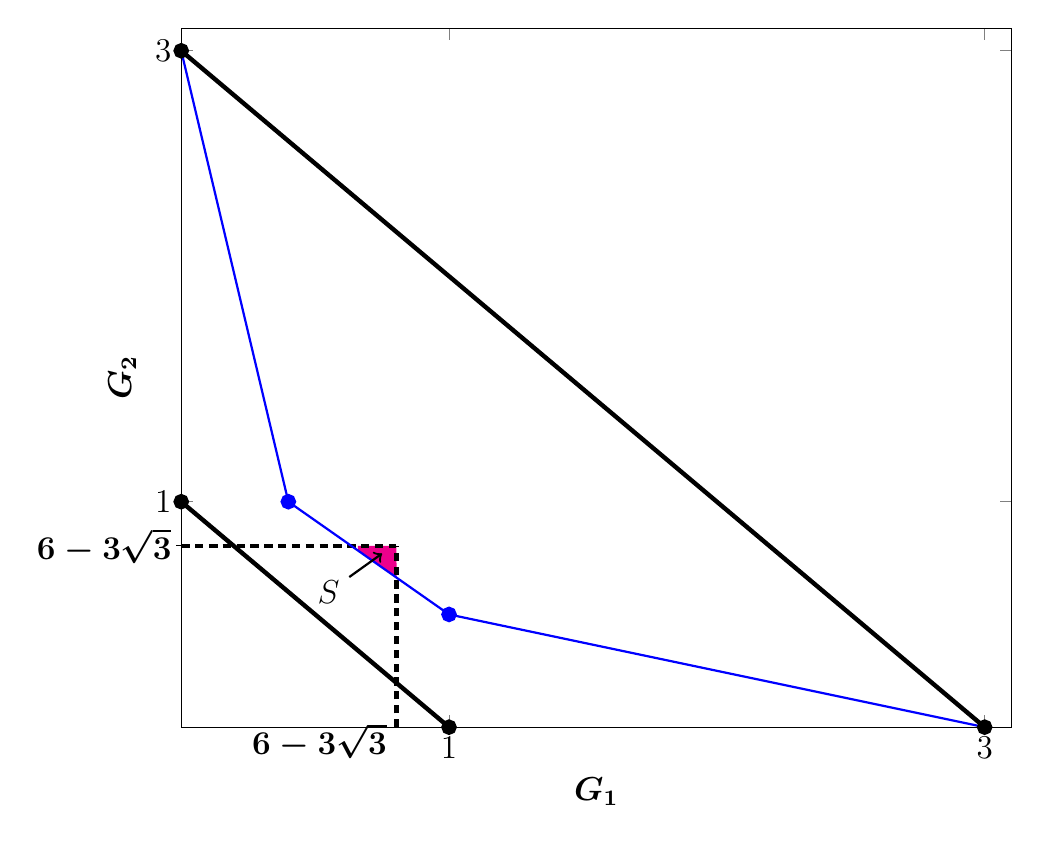
\begin{tikzpicture}
\tikzstyle{every node}=[font=\large]
\begin{axis}[ymax=3.1, ymin=0, xmin=0, xmax=3.1, xlabel= $\boldsymbol{G_1}$, ylabel=$\boldsymbol{G_2}$, xtick={1, 3}, ytick={1, 3},]
    \addlegendimage{red, ultra thick}
    \addlegendimage{blue, ultra thick, dashed}
    \addplot[color=black, ultra thick, mark=*, only marks] coordinates {(0, 3)};
    \addplot[color=black, ultra thick, mark=*, only marks] coordinates {(3, 0)};
    \addplot[color=black, ultra thick, mark=*, only marks] coordinates {(0, 1)};
    \addplot[color=black, ultra thick, mark=*, only marks] coordinates {(1, 0)};
    % \addplot[color=blue, ultra thick, mark=o, only marks] coordinates {(1, 1)};
    \addplot[name path=A, color=black, domain=0:1, ultra thick]{1-x};
    \addplot[name path=B, color=black, domain=0:3, ultra thick]{3-x};
    % \addplot[blue!30] fill between[of=A and B];
    \addplot[name path=C, color=black, densely dashed, ultra thick, domain=0:0.80385]{0.80385};
    \addplot[name path=D, color=black, densely dashed, ultra thick] coordinates {(0.80385, 0) (0.80385, 0.80385)};
    \addplot[color=blue, ultra thick, mark=*, only marks] coordinates {(0.4, 1)}; % (t, 1)
    \addplot[color=blue, ultra thick, mark=*, only marks] coordinates {(1, 0.5)}; % (1, 1-t)
    \addplot[color=blue, thick] coordinates {(0, 3) (0.4, 1)};
    \addplot[name path=E, color=blue, thick] coordinates {(0.4, 1) (1, 0.5)};
    \addplot[color=blue, thick] coordinates {(1, 0.5) (3, 0)};
    \addplot[color=magenta] fill between[of=C and E, soft clip={domain=0.66:0.80385}];
        \addplot[
mark=-,only marks,    
nodes near coords={$\boldsymbol{6-3\sqrt{3}}$},      % Label content
    nodes near coords align={west},     % Align label below the point
    every node near coord/.append style={anchor=east} 
]
coordinates {(0, 0.8038)};
\addplot[
yshift=-5pt, only marks,    
nodes near coords={$\boldsymbol{6-3\sqrt{3}}$},      % Label content
    nodes near coords align={south},     % Align label below the point
    every node near coord/.append style={anchor=east} 
]
coordinates {(0.8038, 0)};
\node[] at (55, 60) (S) {$S$};
\draw[->, thick] (S)--(75, 77);
\end{axis}
\end{tikzpicture}
\end{document}